\section{绝对值函数}
\begin{definition}[绝对值]
设\(x \in \mathbb{R}\),则称函数\[
	f(x) = \left\{ \begin{array}{c}
		x, \quad x \geq 0 \\
		-x, \quad x < 0
	\end{array} \right.
\]为\(x\)的绝对值,
记作\(\abs{x}\).
\end{definition}

\begin{figure}[ht]
	\centering
	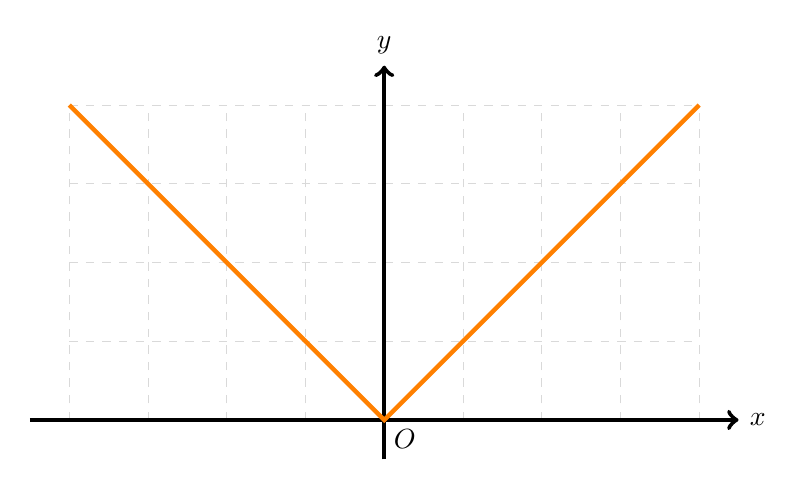
\begin{tikzpicture}
		\draw[help lines, color=gray!30, dashed] (-4,0) grid (4,4);
		\draw[->, ultra thick] (-4.5,0) -- (4.5,0) node[right]{\(x\)};
		\draw[->, ultra thick] (0,-0.5) -- (0,4.5) node[above]{\(y\)};
		\draw (0,0)node[below right]{\(O\)};
		\draw[orange,ultra thick] (-4,4)--(0,0)--(4,4);
	\end{tikzpicture}
	\caption{绝对值函数\(\abs{x}\)的图形}
\end{figure}

\begin{proposition}
设\(a,b\in\mathbb{R}\),
则\(\abs{ab} = \abs{a} \abs{b}\).
\begin{proof}
当\(a=0\)或\(b=0\)时,易见\(\abs{ab} = 0 = \abs{a} \abs{b}\).
当\(a\neq0\)且\(b\neq0\)时,
按照\(a\)和\(b\)的不同取值,列表如下:
\begin{center}
	\begin{tblr}{|*2c|*2{c|}}
		\hline
		&& \(b>0\) & \(b<0\) \\
		&& \(\abs{b}=b\) & \(\abs{b}=-b\) \\ \hline
		\(a>0\) & \(\abs{a}=a\) & \(ab>0,\abs{ab}=ab\) & \(ab<0,\abs{ab}=-ab\) \\ \hline
		\(a<0\) & \(\abs{a}=-a\) & \(ab<0,\abs{ab}=-ab\) & \(ab>0,\abs{ab}=ab\) \\ \hline
	\end{tblr}
\end{center}
由此可知\(\abs{ab} = \abs{a} \abs{b}\)恒成立.
\end{proof}
\end{proposition}

\begin{proposition}
设\(a\)和\(b\)都是实数,
则\begin{gather}
	\min\{a,b\}
	= \frac{a+b}{2}
	- \frac{\abs{a-b}}{2}, \\
	\max\{a,b\}
	= \frac{a+b}{2}
	+ \frac{\abs{a-b}}{2}.
\end{gather}
\begin{proof}
当\(a>b\)时,有\[
	\frac{a+b}{2} - \frac{\abs{a-b}}{2}
	= \frac{a+b}{2} - \frac{a-b}{2}
	= \frac{2b}{2} = b
	= \min\{a,b\},
\]\[
	\frac{a+b}{2} + \frac{\abs{a-b}}{2}
	= \frac{a+b}{2} + \frac{a-b}{2}
	= \frac{2a}{2} = a
	= \max\{a,b\}.
\]
当\(a \leq b\)时,有\[
	\frac{a+b}{2} - \frac{\abs{a-b}}{2}
	= \frac{a+b}{2} - \frac{b-a}{2}
	= \frac{2a}{2} = a
	= \min\{a,b\},
\]\[
	\frac{a+b}{2} + \frac{\abs{a-b}}{2}
	= \frac{a+b}{2} + \frac{b-a}{2}
	= \frac{2b}{2} = b
	= \max\{a,b\}.
	\qedhere
\]
\end{proof}
\end{proposition}
